\documentclass[1p]{elsarticle_modified}
%\bibliographystyle{elsarticle-num}

%\usepackage[colorlinks]{hyperref}
%\usepackage{abbrmath_seonhwa} %\Abb, \Ascr, \Acal ,\Abf, \Afrak
\usepackage{amsfonts}
\usepackage{amssymb}
\usepackage{amsmath}
\usepackage{amsthm}
\usepackage{scalefnt}
\usepackage{amsbsy}
\usepackage{kotex}
\usepackage{caption}
\usepackage{subfig}
\usepackage{color}
\usepackage{graphicx}
\usepackage{xcolor} %% white, black, red, green, blue, cyan, magenta, yellow
\usepackage{float}
\usepackage{setspace}
\usepackage{hyperref}

\usepackage{tikz}
\usetikzlibrary{arrows}

\usepackage{multirow}
\usepackage{array} % fixed length table
\usepackage{hhline}

%%%%%%%%%%%%%%%%%%%%%
\makeatletter
\renewcommand*\env@matrix[1][\arraystretch]{%
	\edef\arraystretch{#1}%
	\hskip -\arraycolsep
	\let\@ifnextchar\new@ifnextchar
	\array{*\c@MaxMatrixCols c}}
\makeatother %https://tex.stackexchange.com/questions/14071/how-can-i-increase-the-line-spacing-in-a-matrix
%%%%%%%%%%%%%%%

\usepackage[normalem]{ulem}

\newcommand{\msout}[1]{\ifmmode\text{\sout{\ensuremath{#1}}}\else\sout{#1}\fi}
%SOURCE: \msout is \stkout macro in https://tex.stackexchange.com/questions/20609/strikeout-in-math-mode

\newcommand{\cancel}[1]{
	\ifmmode
	{\color{red}\msout{#1}}
	\else
	{\color{red}\sout{#1}}
	\fi
}

\newcommand{\add}[1]{
	{\color{blue}\uwave{#1}}
}

\newcommand{\replace}[2]{
	\ifmmode
	{\color{red}\msout{#1}}{\color{blue}\uwave{#2}}
	\else
	{\color{red}\sout{#1}}{\color{blue}\uwave{#2}}
	\fi
}

\newcommand{\Sol}{\mathcal{S}} %segment
\newcommand{\D}{D} %diagram
\newcommand{\A}{\mathcal{A}} %arc


%%%%%%%%%%%%%%%%%%%%%%%%%%%%%5 test

\def\sl{\operatorname{\textup{SL}}(2,\Cbb)}
\def\psl{\operatorname{\textup{PSL}}(2,\Cbb)}
\def\quan{\mkern 1mu \triangleright \mkern 1mu}

\theoremstyle{definition}
\newtheorem{thm}{Theorem}[section]
\newtheorem{prop}[thm]{Proposition}
\newtheorem{lem}[thm]{Lemma}
\newtheorem{ques}[thm]{Question}
\newtheorem{cor}[thm]{Corollary}
\newtheorem{defn}[thm]{Definition}
\newtheorem{exam}[thm]{Example}
\newtheorem{rmk}[thm]{Remark}
\newtheorem{alg}[thm]{Algorithm}

\newcommand{\I}{\sqrt{-1}}
\begin{document}

%\begin{frontmatter}
%
%\title{Boundary parabolic representations of knots up to 8 crossings}
%
%%% Group authors per affiliation:
%\author{Yunhi Cho} 
%\address{Department of Mathematics, University of Seoul, Seoul, Korea}
%\ead{yhcho@uos.ac.kr}
%
%
%\author{Seonhwa Kim} %\fnref{s_kim}}
%\address{Center for Geometry and Physics, Institute for Basic Science, Pohang, 37673, Korea}
%\ead{ryeona17@ibs.re.kr}
%
%\author{Hyuk Kim}
%\address{Department of Mathematical Sciences, Seoul National University, Seoul 08826, Korea}
%\ead{hyukkim@snu.ac.kr}
%
%\author{Seokbeom Yoon}
%\address{Department of Mathematical Sciences, Seoul National University, Seoul, 08826,  Korea}
%\ead{sbyoon15@snu.ac.kr}
%
%\begin{abstract}
%We find all boundary parabolic representation of knots up to 8 crossings.
%
%\end{abstract}
%\begin{keyword}
%    \MSC[2010] 57M25 
%\end{keyword}
%
%\end{frontmatter}

%\linenumbers
%\tableofcontents
%
\newcommand\colored[1]{\textcolor{white}{\rule[-0.35ex]{0.8em}{1.4ex}}\kern-0.8em\color{red} #1}%
%\newcommand\colored[1]{\textcolor{white}{ #1}\kern-2.17ex	\textcolor{white}{ #1}\kern-1.81ex	\textcolor{white}{ #1}\kern-2.15ex\color{red}#1	}

{\Large $\underline{12n_{0022}~(K12n_{0022})}$}

\setlength{\tabcolsep}{10pt}
\renewcommand{\arraystretch}{1.6}
\vspace{1cm}\begin{tabular}{m{100pt}>{\centering\arraybackslash}m{274pt}}
\multirow{5}{120pt}{
	\centering
	\includegraphics[width=112pt]{../../../GIT/diagram.site/Diagrams/png/2111_12n_0022.png}\\
\ \ \ A knot diagram\footnotemark}&
\allowdisplaybreaks
\textbf{Linearized knot diagam} \\
\cline{2-2}
 &
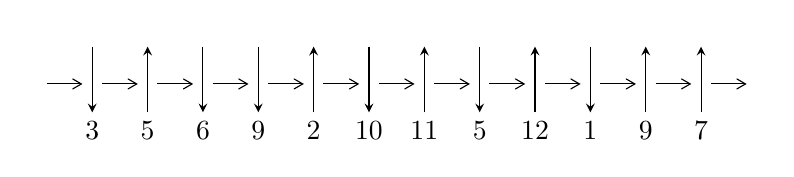
\begin{tikzpicture}[x=20pt, y=17pt]
	% nodes
	\node (C0) at (0, 0) {};
	\node (C1) at (1, 0) {};
	\node (C1U) at (1, +1) {};
	\node (C1D) at (1, -1) {3};

	\node (C2) at (2, 0) {};
	\node (C2U) at (2, +1) {};
	\node (C2D) at (2, -1) {5};

	\node (C3) at (3, 0) {};
	\node (C3U) at (3, +1) {};
	\node (C3D) at (3, -1) {6};

	\node (C4) at (4, 0) {};
	\node (C4U) at (4, +1) {};
	\node (C4D) at (4, -1) {9};

	\node (C5) at (5, 0) {};
	\node (C5U) at (5, +1) {};
	\node (C5D) at (5, -1) {2};

	\node (C6) at (6, 0) {};
	\node (C6U) at (6, +1) {};
	\node (C6D) at (6, -1) {10};

	\node (C7) at (7, 0) {};
	\node (C7U) at (7, +1) {};
	\node (C7D) at (7, -1) {11};

	\node (C8) at (8, 0) {};
	\node (C8U) at (8, +1) {};
	\node (C8D) at (8, -1) {5};

	\node (C9) at (9, 0) {};
	\node (C9U) at (9, +1) {};
	\node (C9D) at (9, -1) {12};

	\node (C10) at (10, 0) {};
	\node (C10U) at (10, +1) {};
	\node (C10D) at (10, -1) {1};

	\node (C11) at (11, 0) {};
	\node (C11U) at (11, +1) {};
	\node (C11D) at (11, -1) {9};

	\node (C12) at (12, 0) {};
	\node (C12U) at (12, +1) {};
	\node (C12D) at (12, -1) {7};
	\node (C13) at (13, 0) {};

	% arrows
	\draw[->,>={angle 60}]
	(C0) edge (C1) (C1) edge (C2) (C2) edge (C3) (C3) edge (C4) (C4) edge (C5) (C5) edge (C6) (C6) edge (C7) (C7) edge (C8) (C8) edge (C9) (C9) edge (C10) (C10) edge (C11) (C11) edge (C12) (C12) edge (C13) ;	\draw[->,>=stealth]
	(C1U) edge (C1D) (C2D) edge (C2U) (C3U) edge (C3D) (C4U) edge (C4D) (C5D) edge (C5U) (C6U) edge (C6D) (C7D) edge (C7U) (C8U) edge (C8D) (C9D) edge (C9U) (C10U) edge (C10D) (C11D) edge (C11U) (C12D) edge (C12U) ;
	\end{tikzpicture} \\
\hhline{~~} \\& 
\textbf{Solving Sequence} \\ \cline{2-2} 
 &
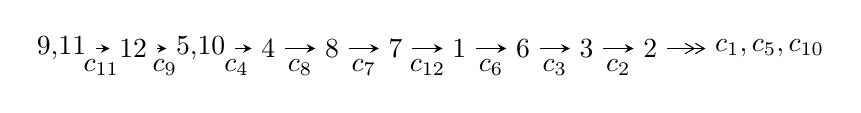
\begin{tikzpicture}[x=23pt, y=7pt]
	% node
	\node (A0) at (-1/8, 0) {9,11};
	\node (A1) at (1, 0) {12};
	\node (A2) at (33/16, 0) {5,10};
	\node (A3) at (25/8, 0) {4};
	\node (A4) at (33/8, 0) {8};
	\node (A5) at (41/8, 0) {7};
	\node (A6) at (49/8, 0) {1};
	\node (A7) at (57/8, 0) {6};
	\node (A8) at (65/8, 0) {3};
	\node (A9) at (73/8, 0) {2};
	\node (C1) at (1/2, -1) {$c_{11}$};
	\node (C2) at (3/2, -1) {$c_{9}$};
	\node (C3) at (21/8, -1) {$c_{4}$};
	\node (C4) at (29/8, -1) {$c_{8}$};
	\node (C5) at (37/8, -1) {$c_{7}$};
	\node (C6) at (45/8, -1) {$c_{12}$};
	\node (C7) at (53/8, -1) {$c_{6}$};
	\node (C8) at (61/8, -1) {$c_{3}$};
	\node (C9) at (69/8, -1) {$c_{2}$};
	\node (A10) at (11, 0) {$c_{1},c_{5},c_{10}$};

	% edge
	\draw[->,>=stealth]	
	(A0) edge (A1) (A1) edge (A2) (A2) edge (A3) (A3) edge (A4) (A4) edge (A5) (A5) edge (A6) (A6) edge (A7) (A7) edge (A8) (A8) edge (A9) ;
	\draw[->>,>={angle 60}]	
	(A9) edge (A10);
\end{tikzpicture} \\ 

\end{tabular} \\

\footnotetext{
The image of knot diagram is generated by the software ``\textbf{Draw programme}" developed by Andrew Bartholomew(\url{http://www.layer8.co.uk/maths/draw/index.htm\#Running-draw}), where we modified some parts for our purpose(\url{https://github.com/CATsTAILs/LinksPainter}).
}\phantom \\ \newline 
\centering \textbf{Ideals for irreducible components\footnotemark of $X_{\text{par}}$} 
 
\begin{align*}
I^u_{1}&=\langle 
2.22558\times10^{224} u^{83}+1.62605\times10^{225} u^{82}+\cdots+2.32318\times10^{225} b+2.05431\times10^{225},\\
\phantom{I^u_{1}}&\phantom{= \langle  }1.34240\times10^{225} u^{83}+9.14747\times10^{225} u^{82}+\cdots+2.32318\times10^{225} a+1.22489\times10^{225},\;u^{84}+7 u^{83}+\cdots+19 u+1\rangle \\
I^u_{2}&=\langle 
- u^4 b- u^3 b+2 u^4+u^2 b+4 u^3+b^2- b- u+2,\;a,\;u^5+u^4-2 u^3- u^2+u-1\rangle \\
I^u_{3}&=\langle 
-2 a^3+b-5 a-1,\;a^4- a^3+3 a^2-2 a+1,\;u-1\rangle \\
\\
\end{align*}
\raggedright * 3 irreducible components of $\dim_{\mathbb{C}}=0$, with total 98 representations.\\
\footnotetext{All coefficients of polynomials are rational numbers. But the coefficients are sometimes approximated in decimal forms when there is not enough margin.}
\newpage
\renewcommand{\arraystretch}{1}
\centering \section*{I. $I^u_{1}= \langle 2.23\times10^{224} u^{83}+1.63\times10^{225} u^{82}+\cdots+2.32\times10^{225} b+2.05\times10^{225},\;1.34\times10^{225} u^{83}+9.15\times10^{225} u^{82}+\cdots+2.32\times10^{225} a+1.22\times10^{225},\;u^{84}+7 u^{83}+\cdots+19 u+1 \rangle$}
\flushleft \textbf{(i) Arc colorings}\\
\begin{tabular}{m{7pt} m{180pt} m{7pt} m{180pt} }
\flushright $a_{9}=$&$\begin{pmatrix}0\\u\end{pmatrix}$ \\
\flushright $a_{11}=$&$\begin{pmatrix}1\\0\end{pmatrix}$ \\
\flushright $a_{12}=$&$\begin{pmatrix}1\\- u^2\end{pmatrix}$ \\
\flushright $a_{5}=$&$\begin{pmatrix}-0.577827 u^{83}-3.93748 u^{82}+\cdots-101.647 u-0.527248\\-0.0957989 u^{83}-0.699925 u^{82}+\cdots-13.0229 u-0.884264\end{pmatrix}$ \\
\flushright $a_{10}=$&$\begin{pmatrix}u\\- u^3+u\end{pmatrix}$ \\
\flushright $a_{4}=$&$\begin{pmatrix}-0.577827 u^{83}-3.93748 u^{82}+\cdots-101.647 u-0.527248\\-0.0821773 u^{83}-0.611145 u^{82}+\cdots-11.5617 u-0.776950\end{pmatrix}$ \\
\flushright $a_{8}=$&$\begin{pmatrix}0.982090 u^{83}+6.78620 u^{82}+\cdots+125.606 u+9.18920\\0.0715056 u^{83}+0.535672 u^{82}+\cdots+11.4628 u+1.15633\end{pmatrix}$ \\
\flushright $a_{7}=$&$\begin{pmatrix}0.910584 u^{83}+6.25053 u^{82}+\cdots+114.143 u+8.03287\\0.0715056 u^{83}+0.535672 u^{82}+\cdots+11.4628 u+1.15633\end{pmatrix}$ \\
\flushright $a_{1}=$&$\begin{pmatrix}0.222432 u^{83}+1.54054 u^{82}+\cdots+4.65720 u+4.57953\\0.0211304 u^{83}+0.0895277 u^{82}+\cdots-0.444083 u+0.205948\end{pmatrix}$ \\
\flushright $a_{6}=$&$\begin{pmatrix}0.860405 u^{83}+5.98086 u^{82}+\cdots+112.669 u+7.91304\\0.116676 u^{83}+0.831091 u^{82}+\cdots+11.4882 u+1.11809\end{pmatrix}$ \\
\flushright $a_{3}=$&$\begin{pmatrix}-0.337224 u^{83}-2.15359 u^{82}+\cdots-80.3989 u+4.87290\\-0.0485546 u^{83}-0.398974 u^{82}+\cdots-10.5681 u-0.387718\end{pmatrix}$ \\
\flushright $a_{2}=$&$\begin{pmatrix}-1.01424 u^{83}-6.93488 u^{82}+\cdots-144.713 u-6.43592\\-0.171241 u^{83}-1.16510 u^{82}+\cdots-12.7424 u-1.08398\end{pmatrix}$\\&\end{tabular}
\flushleft \textbf{(ii) Obstruction class $= -1$}\\~\\
\flushleft \textbf{(iii) Cusp Shapes $= -0.661245 u^{83}-4.69918 u^{82}+\cdots-96.1927 u-11.9327$}\\~\\
\newpage\renewcommand{\arraystretch}{1}
\flushleft \textbf{(iv) u-Polynomials at the component}\newline \\
\begin{tabular}{m{50pt}|m{274pt}}
Crossings & \hspace{64pt}u-Polynomials at each crossing \\
\hline $$\begin{aligned}c_{1}\end{aligned}$$&$\begin{aligned}
&u^{84}+43 u^{83}+\cdots-18 u+1
\end{aligned}$\\
\hline $$\begin{aligned}c_{2},c_{5}\end{aligned}$$&$\begin{aligned}
&u^{84}+7 u^{83}+\cdots+8 u+1
\end{aligned}$\\
\hline $$\begin{aligned}c_{3}\end{aligned}$$&$\begin{aligned}
&u^{84}-7 u^{83}+\cdots+18564 u+47236
\end{aligned}$\\
\hline $$\begin{aligned}c_{4},c_{8}\end{aligned}$$&$\begin{aligned}
&u^{84}+2 u^{83}+\cdots+3072 u+1024
\end{aligned}$\\
\hline $$\begin{aligned}c_{6}\end{aligned}$$&$\begin{aligned}
&u^{84}+u^{83}+\cdots-1664 u+101
\end{aligned}$\\
\hline $$\begin{aligned}c_{7}\end{aligned}$$&$\begin{aligned}
&u^{84}-5 u^{83}+\cdots+78942 u+33589
\end{aligned}$\\
\hline $$\begin{aligned}c_{9},c_{11}\end{aligned}$$&$\begin{aligned}
&u^{84}+7 u^{83}+\cdots+19 u+1
\end{aligned}$\\
\hline $$\begin{aligned}c_{10}\end{aligned}$$&$\begin{aligned}
&u^{84}-13 u^{83}+\cdots+104 u+16
\end{aligned}$\\
\hline $$\begin{aligned}c_{12}\end{aligned}$$&$\begin{aligned}
&u^{84}+4 u^{83}+\cdots+3 u+1
\end{aligned}$\\
\hline
\end{tabular}\\~\\
\newpage\renewcommand{\arraystretch}{1}
\flushleft \textbf{(v) Riley Polynomials at the component}\newline \\
\begin{tabular}{m{50pt}|m{274pt}}
Crossings & \hspace{64pt}Riley Polynomials at each crossing \\
\hline $$\begin{aligned}c_{1}\end{aligned}$$&$\begin{aligned}
&y^{84}+3 y^{83}+\cdots-590 y+1
\end{aligned}$\\
\hline $$\begin{aligned}c_{2},c_{5}\end{aligned}$$&$\begin{aligned}
&y^{84}+43 y^{83}+\cdots-18 y+1
\end{aligned}$\\
\hline $$\begin{aligned}c_{3}\end{aligned}$$&$\begin{aligned}
&y^{84}-37 y^{83}+\cdots-5800852456 y+2231239696
\end{aligned}$\\
\hline $$\begin{aligned}c_{4},c_{8}\end{aligned}$$&$\begin{aligned}
&y^{84}-50 y^{83}+\cdots-22020096 y+1048576
\end{aligned}$\\
\hline $$\begin{aligned}c_{6}\end{aligned}$$&$\begin{aligned}
&y^{84}+69 y^{83}+\cdots-1278338 y+10201
\end{aligned}$\\
\hline $$\begin{aligned}c_{7}\end{aligned}$$&$\begin{aligned}
&y^{84}+85 y^{83}+\cdots-18778069822 y+1128220921
\end{aligned}$\\
\hline $$\begin{aligned}c_{9},c_{11}\end{aligned}$$&$\begin{aligned}
&y^{84}-49 y^{83}+\cdots-211 y+1
\end{aligned}$\\
\hline $$\begin{aligned}c_{10}\end{aligned}$$&$\begin{aligned}
&y^{84}-21 y^{83}+\cdots-19776 y+256
\end{aligned}$\\
\hline $$\begin{aligned}c_{12}\end{aligned}$$&$\begin{aligned}
&y^{84}-24 y^{83}+\cdots+11 y+1
\end{aligned}$\\
\hline
\end{tabular}\\~\\
\newpage\flushleft \textbf{(vi) Complex Volumes and Cusp Shapes}
$$\begin{array}{c|c|c}  
\text{Solutions to }I^u_{1}& \I (\text{vol} + \sqrt{-1}CS) & \text{Cusp shape}\\
 \hline 
\begin{aligned}
u &= \phantom{-}0.972442 + 0.213795 I \\
a &= -1.091770 + 0.371559 I \\
b &= \phantom{-}0.06522 + 2.55411 I\end{aligned}
 & -0.637274 + 0.732588 I & \phantom{-0.000000 } 0 \\ \hline\begin{aligned}
u &= \phantom{-}0.972442 - 0.213795 I \\
a &= -1.091770 - 0.371559 I \\
b &= \phantom{-}0.06522 - 2.55411 I\end{aligned}
 & -0.637274 - 0.732588 I & \phantom{-0.000000 } 0 \\ \hline\begin{aligned}
u &= \phantom{-}1.008760 + 0.011115 I \\
a &= -0.356315 - 0.506244 I \\
b &= -4.87249 - 4.18408 I\end{aligned}
 & \phantom{-}1.40295 - 1.45862 I & \phantom{-0.000000 } 0 \\ \hline\begin{aligned}
u &= \phantom{-}1.008760 - 0.011115 I \\
a &= -0.356315 + 0.506244 I \\
b &= -4.87249 + 4.18408 I\end{aligned}
 & \phantom{-}1.40295 + 1.45862 I & \phantom{-0.000000 } 0 \\ \hline\begin{aligned}
u &= \phantom{-}0.910290 + 0.355435 I \\
a &= \phantom{-}1.315660 - 0.399016 I \\
b &= \phantom{-}0.02342 - 2.05906 I\end{aligned}
 & -4.18720 - 3.29608 I & \phantom{-0.000000 } 0 \\ \hline\begin{aligned}
u &= \phantom{-}0.910290 - 0.355435 I \\
a &= \phantom{-}1.315660 + 0.399016 I \\
b &= \phantom{-}0.02342 + 2.05906 I\end{aligned}
 & -4.18720 + 3.29608 I & \phantom{-0.000000 } 0 \\ \hline\begin{aligned}
u &= -0.320871 + 0.909040 I \\
a &= -1.114210 + 0.444929 I \\
b &= -0.125891 + 0.751460 I\end{aligned}
 & -3.15026 + 4.66896 I & \phantom{-0.000000 } 0 \\ \hline\begin{aligned}
u &= -0.320871 - 0.909040 I \\
a &= -1.114210 - 0.444929 I \\
b &= -0.125891 - 0.751460 I\end{aligned}
 & -3.15026 - 4.66896 I & \phantom{-0.000000 } 0 \\ \hline\begin{aligned}
u &= -0.955077 + 0.022703 I \\
a &= \phantom{-}0.04180 + 1.68922 I \\
b &= -0.014974 + 0.435556 I\end{aligned}
 & \phantom{-}8.34326 - 3.21240 I & \phantom{-0.000000 } 0 \\ \hline\begin{aligned}
u &= -0.955077 - 0.022703 I \\
a &= \phantom{-}0.04180 - 1.68922 I \\
b &= -0.014974 - 0.435556 I\end{aligned}
 & \phantom{-}8.34326 + 3.21240 I & \phantom{-0.000000 } 0\\
 \hline 
 \end{array}$$\newpage$$\begin{array}{c|c|c}  
\text{Solutions to }I^u_{1}& \I (\text{vol} + \sqrt{-1}CS) & \text{Cusp shape}\\
 \hline 
\begin{aligned}
u &= -0.924612 + 0.497424 I \\
a &= \phantom{-}0.734134 - 1.203290 I \\
b &= \phantom{-}0.236759 - 0.476931 I\end{aligned}
 & -1.47667 - 1.22264 I & \phantom{-0.000000 } 0 \\ \hline\begin{aligned}
u &= -0.924612 - 0.497424 I \\
a &= \phantom{-}0.734134 + 1.203290 I \\
b &= \phantom{-}0.236759 + 0.476931 I\end{aligned}
 & -1.47667 + 1.22264 I & \phantom{-0.000000 } 0 \\ \hline\begin{aligned}
u &= \phantom{-}0.331216 + 0.881361 I \\
a &= \phantom{-}0.676599 - 0.353102 I \\
b &= -0.240051 - 0.675771 I\end{aligned}
 & -0.20954 + 2.08673 I & \phantom{-0.000000 } 0 \\ \hline\begin{aligned}
u &= \phantom{-}0.331216 - 0.881361 I \\
a &= \phantom{-}0.676599 + 0.353102 I \\
b &= -0.240051 + 0.675771 I\end{aligned}
 & -0.20954 - 2.08673 I & \phantom{-0.000000 } 0 \\ \hline\begin{aligned}
u &= -0.617703 + 0.685861 I \\
a &= -1.34773 - 1.23740 I \\
b &= \phantom{-}0.162497 - 1.031290 I\end{aligned}
 & -8.44334 - 3.92581 I & \phantom{-0.000000 } 0 \\ \hline\begin{aligned}
u &= -0.617703 - 0.685861 I \\
a &= -1.34773 + 1.23740 I \\
b &= \phantom{-}0.162497 + 1.031290 I\end{aligned}
 & -8.44334 + 3.92581 I & \phantom{-0.000000 } 0 \\ \hline\begin{aligned}
u &= \phantom{-}1.079180 + 0.258468 I \\
a &= \phantom{-}1.109110 - 0.542042 I \\
b &= \phantom{-}0.36270 - 2.45765 I\end{aligned}
 & -3.79074 + 5.18593 I & \phantom{-0.000000 } 0 \\ \hline\begin{aligned}
u &= \phantom{-}1.079180 - 0.258468 I \\
a &= \phantom{-}1.109110 + 0.542042 I \\
b &= \phantom{-}0.36270 + 2.45765 I\end{aligned}
 & -3.79074 - 5.18593 I & \phantom{-0.000000 } 0 \\ \hline\begin{aligned}
u &= \phantom{-}0.993301 + 0.517113 I \\
a &= -0.476198 - 0.466599 I \\
b &= \phantom{-}1.093620 - 0.529398 I\end{aligned}
 & \phantom{-}1.55672 + 3.93406 I & \phantom{-0.000000 } 0 \\ \hline\begin{aligned}
u &= \phantom{-}0.993301 - 0.517113 I \\
a &= -0.476198 + 0.466599 I \\
b &= \phantom{-}1.093620 + 0.529398 I\end{aligned}
 & \phantom{-}1.55672 - 3.93406 I & \phantom{-0.000000 } 0\\
 \hline 
 \end{array}$$\newpage$$\begin{array}{c|c|c}  
\text{Solutions to }I^u_{1}& \I (\text{vol} + \sqrt{-1}CS) & \text{Cusp shape}\\
 \hline 
\begin{aligned}
u &= -1.030100 + 0.473272 I \\
a &= \phantom{-}0.752223 + 1.062450 I \\
b &= -0.26649 + 1.44063 I\end{aligned}
 & -2.21135 - 4.59052 I & \phantom{-0.000000 } 0 \\ \hline\begin{aligned}
u &= -1.030100 - 0.473272 I \\
a &= \phantom{-}0.752223 - 1.062450 I \\
b &= -0.26649 - 1.44063 I\end{aligned}
 & -2.21135 + 4.59052 I & \phantom{-0.000000 } 0 \\ \hline\begin{aligned}
u &= \phantom{-}0.858393 + 0.054295 I \\
a &= -0.165809 - 0.777617 I \\
b &= \phantom{-}2.21383 - 0.21187 I\end{aligned}
 & \phantom{-}0.83780 - 1.60534 I & \phantom{-}11.55428 + 0. I\phantom{ +0.000000I} \\ \hline\begin{aligned}
u &= \phantom{-}0.858393 - 0.054295 I \\
a &= -0.165809 + 0.777617 I \\
b &= \phantom{-}2.21383 + 0.21187 I\end{aligned}
 & \phantom{-}0.83780 + 1.60534 I & \phantom{-}11.55428 + 0. I\phantom{ +0.000000I} \\ \hline\begin{aligned}
u &= -1.058300 + 0.459470 I \\
a &= \phantom{-}1.025540 + 0.596498 I \\
b &= -1.05338 + 1.07754 I\end{aligned}
 & \phantom{-}1.64539 - 2.41566 I & \phantom{-0.000000 } 0 \\ \hline\begin{aligned}
u &= -1.058300 - 0.459470 I \\
a &= \phantom{-}1.025540 - 0.596498 I \\
b &= -1.05338 - 1.07754 I\end{aligned}
 & \phantom{-}1.64539 + 2.41566 I & \phantom{-0.000000 } 0 \\ \hline\begin{aligned}
u &= \phantom{-}1.142540 + 0.177564 I \\
a &= -0.337203 + 0.263085 I \\
b &= \phantom{-}3.94715 + 2.02247 I\end{aligned}
 & \phantom{-}2.34989 - 1.68894 I & \phantom{-0.000000 } 0 \\ \hline\begin{aligned}
u &= \phantom{-}1.142540 - 0.177564 I \\
a &= -0.337203 - 0.263085 I \\
b &= \phantom{-}3.94715 - 2.02247 I\end{aligned}
 & \phantom{-}2.34989 + 1.68894 I & \phantom{-0.000000 } 0 \\ \hline\begin{aligned}
u &= -0.935581 + 0.684978 I \\
a &= -0.673974 - 1.122900 I \\
b &= \phantom{-}0.10781 - 1.52966 I\end{aligned}
 & -7.54628 - 1.28985 I & \phantom{-0.000000 } 0 \\ \hline\begin{aligned}
u &= -0.935581 - 0.684978 I \\
a &= -0.673974 + 1.122900 I \\
b &= \phantom{-}0.10781 + 1.52966 I\end{aligned}
 & -7.54628 + 1.28985 I & \phantom{-0.000000 } 0\\
 \hline 
 \end{array}$$\newpage$$\begin{array}{c|c|c}  
\text{Solutions to }I^u_{1}& \I (\text{vol} + \sqrt{-1}CS) & \text{Cusp shape}\\
 \hline 
\begin{aligned}
u &= -0.646868 + 0.523459 I \\
a &= -1.29135 + 0.69575 I \\
b &= -0.171529 + 0.706893 I\end{aligned}
 & -2.28832 - 2.96266 I & \phantom{-0.000000 } 0 \\ \hline\begin{aligned}
u &= -0.646868 - 0.523459 I \\
a &= -1.29135 - 0.69575 I \\
b &= -0.171529 - 0.706893 I\end{aligned}
 & -2.28832 + 2.96266 I & \phantom{-0.000000 } 0 \\ \hline\begin{aligned}
u &= -1.126650 + 0.469056 I \\
a &= -0.586175 + 0.912908 I \\
b &= -0.242673 + 0.366478 I\end{aligned}
 & \phantom{-}2.64295 - 5.32501 I & \phantom{-0.000000 } 0 \\ \hline\begin{aligned}
u &= -1.126650 - 0.469056 I \\
a &= -0.586175 - 0.912908 I \\
b &= -0.242673 - 0.366478 I\end{aligned}
 & \phantom{-}2.64295 + 5.32501 I & \phantom{-0.000000 } 0 \\ \hline\begin{aligned}
u &= -1.142420 + 0.498662 I \\
a &= -0.708361 - 1.021390 I \\
b &= \phantom{-}0.32261 - 1.53994 I\end{aligned}
 & -4.74130 - 10.12840 I & \phantom{-0.000000 } 0 \\ \hline\begin{aligned}
u &= -1.142420 - 0.498662 I \\
a &= -0.708361 + 1.021390 I \\
b &= \phantom{-}0.32261 + 1.53994 I\end{aligned}
 & -4.74130 + 10.12840 I & \phantom{-0.000000 } 0 \\ \hline\begin{aligned}
u &= \phantom{-}1.194600 + 0.385549 I \\
a &= \phantom{-}0.359098 - 0.436451 I \\
b &= -2.04003 - 1.89368 I\end{aligned}
 & \phantom{-}2.92160 + 2.77404 I & \phantom{-0.000000 } 0 \\ \hline\begin{aligned}
u &= \phantom{-}1.194600 - 0.385549 I \\
a &= \phantom{-}0.359098 + 0.436451 I \\
b &= -2.04003 + 1.89368 I\end{aligned}
 & \phantom{-}2.92160 - 2.77404 I & \phantom{-0.000000 } 0 \\ \hline\begin{aligned}
u &= -0.226720 + 1.234900 I \\
a &= -0.522923 - 0.990090 I \\
b &= -0.02217 - 1.67883 I\end{aligned}
 & -4.54665 + 5.72043 I & \phantom{-0.000000 } 0 \\ \hline\begin{aligned}
u &= -0.226720 - 1.234900 I \\
a &= -0.522923 + 0.990090 I \\
b &= -0.02217 + 1.67883 I\end{aligned}
 & -4.54665 - 5.72043 I & \phantom{-0.000000 } 0\\
 \hline 
 \end{array}$$\newpage$$\begin{array}{c|c|c}  
\text{Solutions to }I^u_{1}& \I (\text{vol} + \sqrt{-1}CS) & \text{Cusp shape}\\
 \hline 
\begin{aligned}
u &= -1.153780 + 0.515980 I \\
a &= -0.859747 - 0.652054 I \\
b &= \phantom{-}1.11954 - 1.39330 I\end{aligned}
 & \phantom{-}2.03077 - 8.41785 I & \phantom{-0.000000 } 0 \\ \hline\begin{aligned}
u &= -1.153780 - 0.515980 I \\
a &= -0.859747 + 0.652054 I \\
b &= \phantom{-}1.11954 + 1.39330 I\end{aligned}
 & \phantom{-}2.03077 + 8.41785 I & \phantom{-0.000000 } 0 \\ \hline\begin{aligned}
u &= -0.190457 + 0.689630 I \\
a &= -0.255146 - 1.215230 I \\
b &= -0.34868 - 1.70071 I\end{aligned}
 & -0.72347 + 3.79694 I & -4.78687 - 5.26590 I \\ \hline\begin{aligned}
u &= -0.190457 - 0.689630 I \\
a &= -0.255146 + 1.215230 I \\
b &= -0.34868 + 1.70071 I\end{aligned}
 & -0.72347 - 3.79694 I & -4.78687 + 5.26590 I \\ \hline\begin{aligned}
u &= -0.280053 + 0.652017 I \\
a &= -1.46834 - 1.72562 I \\
b &= -0.225602 - 0.904495 I\end{aligned}
 & -7.27588 + 5.64053 I & -4.23717 - 1.44618 I \\ \hline\begin{aligned}
u &= -0.280053 - 0.652017 I \\
a &= -1.46834 + 1.72562 I \\
b &= -0.225602 + 0.904495 I\end{aligned}
 & -7.27588 - 5.64053 I & -4.23717 + 1.44618 I \\ \hline\begin{aligned}
u &= -0.413220 + 1.230540 I \\
a &= \phantom{-}0.552234 + 1.040430 I \\
b &= \phantom{-}0.04555 + 1.65819 I\end{aligned}
 & -9.11776 + 1.81197 I & \phantom{-0.000000 } 0 \\ \hline\begin{aligned}
u &= -0.413220 - 1.230540 I \\
a &= \phantom{-}0.552234 - 1.040430 I \\
b &= \phantom{-}0.04555 - 1.65819 I\end{aligned}
 & -9.11776 - 1.81197 I & \phantom{-0.000000 } 0 \\ \hline\begin{aligned}
u &= \phantom{-}1.258140 + 0.371030 I \\
a &= \phantom{-}0.447345 + 0.321206 I \\
b &= -0.744087 + 0.186455 I\end{aligned}
 & \phantom{-}2.97676 + 0.06912 I & \phantom{-0.000000 } 0 \\ \hline\begin{aligned}
u &= \phantom{-}1.258140 - 0.371030 I \\
a &= \phantom{-}0.447345 - 0.321206 I \\
b &= -0.744087 - 0.186455 I\end{aligned}
 & \phantom{-}2.97676 - 0.06912 I & \phantom{-0.000000 } 0\\
 \hline 
 \end{array}$$\newpage$$\begin{array}{c|c|c}  
\text{Solutions to }I^u_{1}& \I (\text{vol} + \sqrt{-1}CS) & \text{Cusp shape}\\
 \hline 
\begin{aligned}
u &= -1.173850 + 0.596639 I \\
a &= \phantom{-}0.760441 - 0.817940 I \\
b &= \phantom{-}0.321304 - 0.359548 I\end{aligned}
 & -0.55121 - 10.15270 I & \phantom{-0.000000 } 0 \\ \hline\begin{aligned}
u &= -1.173850 - 0.596639 I \\
a &= \phantom{-}0.760441 + 0.817940 I \\
b &= \phantom{-}0.321304 + 0.359548 I\end{aligned}
 & -0.55121 + 10.15270 I & \phantom{-0.000000 } 0 \\ \hline\begin{aligned}
u &= -0.432278 + 0.520555 I \\
a &= \phantom{-}1.72365 + 1.42967 I \\
b &= \phantom{-}0.019219 + 0.763148 I\end{aligned}
 & -3.91699 + 0.49402 I & -1.75716 + 2.00639 I \\ \hline\begin{aligned}
u &= -0.432278 - 0.520555 I \\
a &= \phantom{-}1.72365 - 1.42967 I \\
b &= \phantom{-}0.019219 - 0.763148 I\end{aligned}
 & -3.91699 - 0.49402 I & -1.75716 - 2.00639 I \\ \hline\begin{aligned}
u &= \phantom{-}1.35490\phantom{ +0.000000I} \\
a &= \phantom{-}0.339763\phantom{ +0.000000I} \\
b &= -0.449694\phantom{ +0.000000I}\end{aligned}
 & \phantom{-}2.55442\phantom{ +0.000000I} & \phantom{-0.000000 } 0 \\ \hline\begin{aligned}
u &= -0.198732 + 1.355280 I \\
a &= \phantom{-}0.556728 + 0.968007 I \\
b &= \phantom{-}0.00784 + 1.65359 I\end{aligned}
 & -7.54281 + 10.87570 I & \phantom{-0.000000 } 0 \\ \hline\begin{aligned}
u &= -0.198732 - 1.355280 I \\
a &= \phantom{-}0.556728 - 0.968007 I \\
b &= \phantom{-}0.00784 - 1.65359 I\end{aligned}
 & -7.54281 - 10.87570 I & \phantom{-0.000000 } 0 \\ \hline\begin{aligned}
u &= -1.24156 + 0.72441 I \\
a &= \phantom{-}0.727402 + 0.901724 I \\
b &= -0.73376 + 1.74424 I\end{aligned}
 & -6.44809 - 8.61020 I & \phantom{-0.000000 } 0 \\ \hline\begin{aligned}
u &= -1.24156 - 0.72441 I \\
a &= \phantom{-}0.727402 - 0.901724 I \\
b &= -0.73376 - 1.74424 I\end{aligned}
 & -6.44809 + 8.61020 I & \phantom{-0.000000 } 0 \\ \hline\begin{aligned}
u &= -1.44705 + 0.17137 I \\
a &= \phantom{-}0.315816 + 0.194686 I \\
b &= \phantom{-}0.118682 + 0.118584 I\end{aligned}
 & \phantom{-}5.61123 - 2.65441 I & \phantom{-0.000000 } 0\\
 \hline 
 \end{array}$$\newpage$$\begin{array}{c|c|c}  
\text{Solutions to }I^u_{1}& \I (\text{vol} + \sqrt{-1}CS) & \text{Cusp shape}\\
 \hline 
\begin{aligned}
u &= -1.44705 - 0.17137 I \\
a &= \phantom{-}0.315816 - 0.194686 I \\
b &= \phantom{-}0.118682 - 0.118584 I\end{aligned}
 & \phantom{-}5.61123 + 2.65441 I & \phantom{-0.000000 } 0 \\ \hline\begin{aligned}
u &= \phantom{-}1.18182 + 0.87280 I \\
a &= \phantom{-}0.462410 - 0.603044 I \\
b &= -0.84076 - 1.49220 I\end{aligned}
 & \phantom{-}0.99043 + 3.63889 I & \phantom{-0.000000 } 0 \\ \hline\begin{aligned}
u &= \phantom{-}1.18182 - 0.87280 I \\
a &= \phantom{-}0.462410 + 0.603044 I \\
b &= -0.84076 + 1.49220 I\end{aligned}
 & \phantom{-}0.99043 - 3.63889 I & \phantom{-0.000000 } 0 \\ \hline\begin{aligned}
u &= -1.45343 + 0.26296 I \\
a &= -0.344788 + 0.135869 I \\
b &= -0.165511 + 0.031545 I\end{aligned}
 & \phantom{-}5.71423 - 6.06522 I & \phantom{-0.000000 } 0 \\ \hline\begin{aligned}
u &= -1.45343 - 0.26296 I \\
a &= -0.344788 - 0.135869 I \\
b &= -0.165511 - 0.031545 I\end{aligned}
 & \phantom{-}5.71423 + 6.06522 I & \phantom{-0.000000 } 0 \\ \hline\begin{aligned}
u &= -1.32402 + 0.65852 I \\
a &= -0.637359 - 0.834221 I \\
b &= \phantom{-}0.86308 - 1.90054 I\end{aligned}
 & -1.06531 - 12.31450 I & \phantom{-0.000000 } 0 \\ \hline\begin{aligned}
u &= -1.32402 - 0.65852 I \\
a &= -0.637359 + 0.834221 I \\
b &= \phantom{-}0.86308 + 1.90054 I\end{aligned}
 & -1.06531 + 12.31450 I & \phantom{-0.000000 } 0 \\ \hline\begin{aligned}
u &= \phantom{-}0.99893 + 1.09943 I \\
a &= -0.550292 + 0.618639 I \\
b &= \phantom{-}0.56906 + 1.29599 I\end{aligned}
 & -2.69617 + 0.11948 I & \phantom{-0.000000 } 0 \\ \hline\begin{aligned}
u &= \phantom{-}0.99893 - 1.09943 I \\
a &= -0.550292 - 0.618639 I \\
b &= \phantom{-}0.56906 - 1.29599 I\end{aligned}
 & -2.69617 - 0.11948 I & \phantom{-0.000000 } 0 \\ \hline\begin{aligned}
u &= -0.383297 + 0.340658 I \\
a &= \phantom{-}0.66058 + 1.72839 I \\
b &= \phantom{-}0.333450 + 1.212380 I\end{aligned}
 & -0.303408 - 1.335140 I & -3.78742 + 3.57340 I\\
 \hline 
 \end{array}$$\newpage$$\begin{array}{c|c|c}  
\text{Solutions to }I^u_{1}& \I (\text{vol} + \sqrt{-1}CS) & \text{Cusp shape}\\
 \hline 
\begin{aligned}
u &= -0.383297 - 0.340658 I \\
a &= \phantom{-}0.66058 - 1.72839 I \\
b &= \phantom{-}0.333450 - 1.212380 I\end{aligned}
 & -0.303408 + 1.335140 I & -3.78742 - 3.57340 I \\ \hline\begin{aligned}
u &= -1.37417 + 0.68442 I \\
a &= \phantom{-}0.588585 + 0.869316 I \\
b &= -0.79291 + 1.99045 I\end{aligned}
 & -3.7955 - 17.8954 I & \phantom{-0.000000 } 0 \\ \hline\begin{aligned}
u &= -1.37417 - 0.68442 I \\
a &= \phantom{-}0.588585 - 0.869316 I \\
b &= -0.79291 - 1.99045 I\end{aligned}
 & -3.7955 + 17.8954 I & \phantom{-0.000000 } 0 \\ \hline\begin{aligned}
u &= -0.056966 + 0.445178 I \\
a &= \phantom{-}1.48669 + 0.28338 I \\
b &= \phantom{-}0.203441 - 0.603272 I\end{aligned}
 & -0.081645 + 1.388350 I & -0.20547 - 3.77437 I \\ \hline\begin{aligned}
u &= -0.056966 - 0.445178 I \\
a &= \phantom{-}1.48669 - 0.28338 I \\
b &= \phantom{-}0.203441 + 0.603272 I\end{aligned}
 & -0.081645 - 1.388350 I & -0.20547 + 3.77437 I \\ \hline\begin{aligned}
u &= \phantom{-}1.55444\phantom{ +0.000000I} \\
a &= \phantom{-}0.508397\phantom{ +0.000000I} \\
b &= -0.418678\phantom{ +0.000000I}\end{aligned}
 & \phantom{-}2.51357\phantom{ +0.000000I} & \phantom{-0.000000 } 0 \\ \hline\begin{aligned}
u &= \phantom{-}1.30994 + 1.00098 I \\
a &= -0.459489 + 0.660570 I \\
b &= \phantom{-}0.66060 + 1.60930 I\end{aligned}
 & -1.81006 + 8.25159 I & \phantom{-0.000000 } 0 \\ \hline\begin{aligned}
u &= \phantom{-}1.30994 - 1.00098 I \\
a &= -0.459489 - 0.660570 I \\
b &= \phantom{-}0.66060 - 1.60930 I\end{aligned}
 & -1.81006 - 8.25159 I & \phantom{-0.000000 } 0 \\ \hline\begin{aligned}
u &= \phantom{-}0.172995 + 0.034028 I \\
a &= -1.87202 + 3.59277 I \\
b &= \phantom{-}0.345343 - 0.709443 I\end{aligned}
 & -0.194651 + 1.319340 I & -1.46532 - 4.00362 I \\ \hline\begin{aligned}
u &= \phantom{-}0.172995 - 0.034028 I \\
a &= -1.87202 - 3.59277 I \\
b &= \phantom{-}0.345343 + 0.709443 I\end{aligned}
 & -0.194651 - 1.319340 I & -1.46532 + 4.00362 I\\
 \hline 
 \end{array}$$\newpage$$\begin{array}{c|c|c}  
\text{Solutions to }I^u_{1}& \I (\text{vol} + \sqrt{-1}CS) & \text{Cusp shape}\\
 \hline 
\begin{aligned}
u &= \phantom{-}1.82009 + 0.15092 I \\
a &= -0.657590 - 0.068438 I \\
b &= \phantom{-}0.287435 - 0.079406 I\end{aligned}
 & -0.33247 - 3.91395 I & \phantom{-0.000000 } 0 \\ \hline\begin{aligned}
u &= \phantom{-}1.82009 - 0.15092 I \\
a &= -0.657590 + 0.068438 I \\
b &= \phantom{-}0.287435 + 0.079406 I\end{aligned}
 & -0.33247 + 3.91395 I & \phantom{-0.000000 } 0 \\ \hline\begin{aligned}
u &= -0.0795493 + 0.0409515 I \\
a &= \phantom{-}7.05665 - 2.72768 I \\
b &= \phantom{-}0.405023 - 0.635618 I\end{aligned}
 & -0.176677 + 1.378470 I & -2.64856 - 4.43072 I \\ \hline\begin{aligned}
u &= -0.0795493 - 0.0409515 I \\
a &= \phantom{-}7.05665 + 2.72768 I \\
b &= \phantom{-}0.405023 + 0.635618 I\end{aligned}
 & -0.176677 - 1.378470 I & -2.64856 + 4.43072 I\\
 \hline 
 \end{array}$$\newpage\newpage\renewcommand{\arraystretch}{1}
\centering \section*{II. $I^u_{2}= \langle - u^4 b+2 u^4+\cdots- b+2,\;a,\;u^5+u^4-2 u^3- u^2+u-1 \rangle$}
\flushleft \textbf{(i) Arc colorings}\\
\begin{tabular}{m{7pt} m{180pt} m{7pt} m{180pt} }
\flushright $a_{9}=$&$\begin{pmatrix}0\\u\end{pmatrix}$ \\
\flushright $a_{11}=$&$\begin{pmatrix}1\\0\end{pmatrix}$ \\
\flushright $a_{12}=$&$\begin{pmatrix}1\\- u^2\end{pmatrix}$ \\
\flushright $a_{5}=$&$\begin{pmatrix}0\\b\end{pmatrix}$ \\
\flushright $a_{10}=$&$\begin{pmatrix}u\\- u^3+u\end{pmatrix}$ \\
\flushright $a_{4}=$&$\begin{pmatrix}0\\b\end{pmatrix}$ \\
\flushright $a_{8}=$&$\begin{pmatrix}0\\u\end{pmatrix}$ \\
\flushright $a_{7}=$&$\begin{pmatrix}- u\\u\end{pmatrix}$ \\
\flushright $a_{1}=$&$\begin{pmatrix}- u^4+u^2+1\\u^4-2 u^2\end{pmatrix}$ \\
\flushright $a_{6}=$&$\begin{pmatrix}u^4- u^2-1\\- u^4+2 u^2\end{pmatrix}$ \\
\flushright $a_{3}=$&$\begin{pmatrix}u^4 b- u^3 b-2 u^2 b+3 b u- b\\- b u+2 b\end{pmatrix}$ \\
\flushright $a_{2}=$&$\begin{pmatrix}u^4 b- u^3 b-2 u^2 b+3 b u- b\\- u^4- u^3- b u+u^2+2 b-1\end{pmatrix}$\\&\end{tabular}
\flushleft \textbf{(ii) Obstruction class $= 1$}\\~\\
\flushleft \textbf{(iii) Cusp Shapes $= -8 u^4 b+5 u^3 b- u^4+9 u^2 b+u^3-6 b u-2 u^2+6 b-7 u+3$}\\~\\
\newpage\renewcommand{\arraystretch}{1}
\flushleft \textbf{(iv) u-Polynomials at the component}\newline \\
\begin{tabular}{m{50pt}|m{274pt}}
Crossings & \hspace{64pt}u-Polynomials at each crossing \\
\hline $$\begin{aligned}c_{1},c_{3},c_{5}\end{aligned}$$&$\begin{aligned}
&(u^2- u+1)^5
\end{aligned}$\\
\hline $$\begin{aligned}c_{2}\end{aligned}$$&$\begin{aligned}
&(u^2+u+1)^5
\end{aligned}$\\
\hline $$\begin{aligned}c_{4},c_{8}\end{aligned}$$&$\begin{aligned}
&u^{10}
\end{aligned}$\\
\hline $$\begin{aligned}c_{6},c_{10}\end{aligned}$$&$\begin{aligned}
&(u^5+u^4+2 u^3+u^2+u+1)^2
\end{aligned}$\\
\hline $$\begin{aligned}c_{7},c_{9}\end{aligned}$$&$\begin{aligned}
&(u^5- u^4-2 u^3+u^2+u+1)^2
\end{aligned}$\\
\hline $$\begin{aligned}c_{11}\end{aligned}$$&$\begin{aligned}
&(u^5+u^4-2 u^3- u^2+u-1)^2
\end{aligned}$\\
\hline $$\begin{aligned}c_{12}\end{aligned}$$&$\begin{aligned}
&(u^5-3 u^4+4 u^3- u^2- u+1)^2
\end{aligned}$\\
\hline
\end{tabular}\\~\\
\newpage\renewcommand{\arraystretch}{1}
\flushleft \textbf{(v) Riley Polynomials at the component}\newline \\
\begin{tabular}{m{50pt}|m{274pt}}
Crossings & \hspace{64pt}Riley Polynomials at each crossing \\
\hline $$\begin{aligned}c_{1},c_{2},c_{3}\\c_{5}\end{aligned}$$&$\begin{aligned}
&(y^2+y+1)^5
\end{aligned}$\\
\hline $$\begin{aligned}c_{4},c_{8}\end{aligned}$$&$\begin{aligned}
&y^{10}
\end{aligned}$\\
\hline $$\begin{aligned}c_{6},c_{10}\end{aligned}$$&$\begin{aligned}
&(y^5+3 y^4+4 y^3+y^2- y-1)^2
\end{aligned}$\\
\hline $$\begin{aligned}c_{7},c_{9},c_{11}\end{aligned}$$&$\begin{aligned}
&(y^5-5 y^4+8 y^3-3 y^2- y-1)^2
\end{aligned}$\\
\hline $$\begin{aligned}c_{12}\end{aligned}$$&$\begin{aligned}
&(y^5- y^4+8 y^3-3 y^2+3 y-1)^2
\end{aligned}$\\
\hline
\end{tabular}\\~\\
\newpage\flushleft \textbf{(vi) Complex Volumes and Cusp Shapes}
$$\begin{array}{c|c|c}  
\text{Solutions to }I^u_{2}& \I (\text{vol} + \sqrt{-1}CS) & \text{Cusp shape}\\
 \hline 
\begin{aligned}
u &= \phantom{-}1.21774\phantom{ +0.000000I} \\
a &= \phantom{-0.000000 } 0 \\
b &= \phantom{-}1.76091 + 3.04998 I\end{aligned}
 & \phantom{-}2.40108 - 2.02988 I & -2.76075 + 10.60420 I \\ \hline\begin{aligned}
u &= \phantom{-}1.21774\phantom{ +0.000000I} \\
a &= \phantom{-0.000000 } 0 \\
b &= \phantom{-}1.76091 - 3.04998 I\end{aligned}
 & \phantom{-}2.40108 + 2.02988 I & -2.76075 - 10.60420 I \\ \hline\begin{aligned}
u &= \phantom{-}0.309916 + 0.549911 I \\
a &= \phantom{-0.000000 } 0 \\
b &= \phantom{-}0.864485 + 0.518603 I\end{aligned}
 & \phantom{-}0.329100 - 0.499304 I & \phantom{-}2.01870 - 2.82203 I \\ \hline\begin{aligned}
u &= \phantom{-}0.309916 + 0.549911 I \\
a &= \phantom{-0.000000 } 0 \\
b &= \phantom{-}0.016881 - 1.007970 I\end{aligned}
 & \phantom{-}0.32910 + 3.56046 I & \phantom{-}1.95395 - 6.01185 I \\ \hline\begin{aligned}
u &= \phantom{-}0.309916 - 0.549911 I \\
a &= \phantom{-0.000000 } 0 \\
b &= \phantom{-}0.864485 - 0.518603 I\end{aligned}
 & \phantom{-}0.329100 + 0.499304 I & \phantom{-}2.01870 + 2.82203 I \\ \hline\begin{aligned}
u &= \phantom{-}0.309916 - 0.549911 I \\
a &= \phantom{-0.000000 } 0 \\
b &= \phantom{-}0.016881 + 1.007970 I\end{aligned}
 & \phantom{-}0.32910 - 3.56046 I & \phantom{-}1.95395 + 6.01185 I \\ \hline\begin{aligned}
u &= -1.41878 + 0.21917 I \\
a &= \phantom{-0.000000 } 0 \\
b &= \phantom{-}0.369732 - 0.377747 I\end{aligned}
 & \phantom{-}5.87256 - 6.43072 I & \phantom{-}6.8570 + 13.9114 I \\ \hline\begin{aligned}
u &= -1.41878 + 0.21917 I \\
a &= \phantom{-0.000000 } 0 \\
b &= -0.512005 - 0.131324 I\end{aligned}
 & \phantom{-}5.87256 - 2.37095 I & \phantom{-}9.93110 - 5.20350 I \\ \hline\begin{aligned}
u &= -1.41878 - 0.21917 I \\
a &= \phantom{-0.000000 } 0 \\
b &= \phantom{-}0.369732 + 0.377747 I\end{aligned}
 & \phantom{-}5.87256 + 6.43072 I & \phantom{-}6.8570 - 13.9114 I \\ \hline\begin{aligned}
u &= -1.41878 - 0.21917 I \\
a &= \phantom{-0.000000 } 0 \\
b &= -0.512005 + 0.131324 I\end{aligned}
 & \phantom{-}5.87256 + 2.37095 I & \phantom{-}9.93110 + 5.20350 I\\
 \hline 
 \end{array}$$\newpage\newpage\renewcommand{\arraystretch}{1}
\centering \section*{III. $I^u_{3}= \langle -2 a^3+b-5 a-1,\;a^4- a^3+3 a^2-2 a+1,\;u-1 \rangle$}
\flushleft \textbf{(i) Arc colorings}\\
\begin{tabular}{m{7pt} m{180pt} m{7pt} m{180pt} }
\flushright $a_{9}=$&$\begin{pmatrix}0\\1\end{pmatrix}$ \\
\flushright $a_{11}=$&$\begin{pmatrix}1\\0\end{pmatrix}$ \\
\flushright $a_{12}=$&$\begin{pmatrix}1\\-1\end{pmatrix}$ \\
\flushright $a_{5}=$&$\begin{pmatrix}a\\2 a^3+5 a+1\end{pmatrix}$ \\
\flushright $a_{10}=$&$\begin{pmatrix}1\\0\end{pmatrix}$ \\
\flushright $a_{4}=$&$\begin{pmatrix}a\\2 a^3+4 a+1\end{pmatrix}$ \\
\flushright $a_{8}=$&$\begin{pmatrix}a^2\\2 a^3- a^2+5 a-1\end{pmatrix}$ \\
\flushright $a_{7}=$&$\begin{pmatrix}-2 a^3+2 a^2-5 a+1\\2 a^3- a^2+5 a-1\end{pmatrix}$ \\
\flushright $a_{1}=$&$\begin{pmatrix}- a^3+3 a^2-2 a+1\\0\end{pmatrix}$ \\
\flushright $a_{6}=$&$\begin{pmatrix}a^2\\2 a^3- a^2+5 a-1\end{pmatrix}$ \\
\flushright $a_{3}=$&$\begin{pmatrix}a^3+a^2+1\\a^3+a^2+2 a+3\end{pmatrix}$ \\
\flushright $a_{2}=$&$\begin{pmatrix}a^3+a\\2 a^3- a^2+5 a-1\end{pmatrix}$\\&\end{tabular}
\flushleft \textbf{(ii) Obstruction class $= 1$}\\~\\
\flushleft \textbf{(iii) Cusp Shapes $= -15 a^3+3 a^2-46 a+36$}\\~\\
\newpage\renewcommand{\arraystretch}{1}
\flushleft \textbf{(iv) u-Polynomials at the component}\newline \\
\begin{tabular}{m{50pt}|m{274pt}}
Crossings & \hspace{64pt}u-Polynomials at each crossing \\
\hline $$\begin{aligned}c_{1},c_{4}\end{aligned}$$&$\begin{aligned}
&u^4- u^3+3 u^2-2 u+1
\end{aligned}$\\
\hline $$\begin{aligned}c_{2}\end{aligned}$$&$\begin{aligned}
&u^4- u^3+u^2+1
\end{aligned}$\\
\hline $$\begin{aligned}c_{3}\end{aligned}$$&$\begin{aligned}
&u^4+u^3+5 u^2- u+2
\end{aligned}$\\
\hline $$\begin{aligned}c_{5}\end{aligned}$$&$\begin{aligned}
&u^4+u^3+u^2+1
\end{aligned}$\\
\hline $$\begin{aligned}c_{6},c_{7}\end{aligned}$$&$\begin{aligned}
&u^4+2 u^3+7 u^2+5 u+1
\end{aligned}$\\
\hline $$\begin{aligned}c_{8}\end{aligned}$$&$\begin{aligned}
&u^4+u^3+3 u^2+2 u+1
\end{aligned}$\\
\hline $$\begin{aligned}c_{9}\end{aligned}$$&$\begin{aligned}
&(u+1)^4
\end{aligned}$\\
\hline $$\begin{aligned}c_{10}\end{aligned}$$&$\begin{aligned}
&u^4
\end{aligned}$\\
\hline $$\begin{aligned}c_{11}\end{aligned}$$&$\begin{aligned}
&(u-1)^4
\end{aligned}$\\
\hline $$\begin{aligned}c_{12}\end{aligned}$$&$\begin{aligned}
&u^4+5 u^3+7 u^2+2 u+1
\end{aligned}$\\
\hline
\end{tabular}\\~\\
\newpage\renewcommand{\arraystretch}{1}
\flushleft \textbf{(v) Riley Polynomials at the component}\newline \\
\begin{tabular}{m{50pt}|m{274pt}}
Crossings & \hspace{64pt}Riley Polynomials at each crossing \\
\hline $$\begin{aligned}c_{1},c_{4},c_{8}\end{aligned}$$&$\begin{aligned}
&y^4+5 y^3+7 y^2+2 y+1
\end{aligned}$\\
\hline $$\begin{aligned}c_{2},c_{5}\end{aligned}$$&$\begin{aligned}
&y^4+y^3+3 y^2+2 y+1
\end{aligned}$\\
\hline $$\begin{aligned}c_{3}\end{aligned}$$&$\begin{aligned}
&y^4+9 y^3+31 y^2+19 y+4
\end{aligned}$\\
\hline $$\begin{aligned}c_{6},c_{7}\end{aligned}$$&$\begin{aligned}
&y^4+10 y^3+31 y^2-11 y+1
\end{aligned}$\\
\hline $$\begin{aligned}c_{9},c_{11}\end{aligned}$$&$\begin{aligned}
&(y-1)^4
\end{aligned}$\\
\hline $$\begin{aligned}c_{10}\end{aligned}$$&$\begin{aligned}
&y^4
\end{aligned}$\\
\hline $$\begin{aligned}c_{12}\end{aligned}$$&$\begin{aligned}
&y^4-11 y^3+31 y^2+10 y+1
\end{aligned}$\\
\hline
\end{tabular}\\~\\
\newpage\flushleft \textbf{(vi) Complex Volumes and Cusp Shapes}
$$\begin{array}{c|c|c}  
\text{Solutions to }I^u_{3}& \I (\text{vol} + \sqrt{-1}CS) & \text{Cusp shape}\\
 \hline 
\begin{aligned}
u &= \phantom{-}1.00000\phantom{ +0.000000I} \\
a &= \phantom{-}0.395123 + 0.506844 I \\
b &= \phantom{-}2.48997 + 2.74859 I\end{aligned}
 & \phantom{-}1.43393 - 1.41510 I & \phantom{-}21.1644 - 23.7210 I \\ \hline\begin{aligned}
u &= \phantom{-}1.00000\phantom{ +0.000000I} \\
a &= \phantom{-}0.395123 - 0.506844 I \\
b &= \phantom{-}2.48997 - 2.74859 I\end{aligned}
 & \phantom{-}1.43393 + 1.41510 I & \phantom{-}21.1644 + 23.7210 I \\ \hline\begin{aligned}
u &= \phantom{-}1.00000\phantom{ +0.000000I} \\
a &= \phantom{-}0.10488 + 1.55249 I \\
b &= \phantom{-}0.010029 + 0.381188 I\end{aligned}
 & \phantom{-}8.43568 - 3.16396 I & \phantom{-}35.3356 - 15.0782 I \\ \hline\begin{aligned}
u &= \phantom{-}1.00000\phantom{ +0.000000I} \\
a &= \phantom{-}0.10488 - 1.55249 I \\
b &= \phantom{-}0.010029 - 0.381188 I\end{aligned}
 & \phantom{-}8.43568 + 3.16396 I & \phantom{-}35.3356 + 15.0782 I\\
 \hline 
 \end{array}$$\newpage
\newpage\renewcommand{\arraystretch}{1}
\centering \section*{ IV. u-Polynomials}
\begin{tabular}{m{50pt}|m{274pt}}
Crossings & \hspace{64pt}u-Polynomials at each crossing \\
\hline $$\begin{aligned}c_{1}\end{aligned}$$&$\begin{aligned}
&((u^2- u+1)^5)(u^4- u^3+3 u^2-2 u+1)(u^{84}+43 u^{83}+\cdots-18 u+1)
\end{aligned}$\\
\hline $$\begin{aligned}c_{2}\end{aligned}$$&$\begin{aligned}
&((u^2+u+1)^5)(u^4- u^3+u^2+1)(u^{84}+7 u^{83}+\cdots+8 u+1)
\end{aligned}$\\
\hline $$\begin{aligned}c_{3}\end{aligned}$$&$\begin{aligned}
&(u^2- u+1)^5(u^4+u^3+5 u^2- u+2)\\
&\cdot(u^{84}-7 u^{83}+\cdots+18564 u+47236)
\end{aligned}$\\
\hline $$\begin{aligned}c_{4}\end{aligned}$$&$\begin{aligned}
&u^{10}(u^4- u^3+3 u^2-2 u+1)(u^{84}+2 u^{83}+\cdots+3072 u+1024)
\end{aligned}$\\
\hline $$\begin{aligned}c_{5}\end{aligned}$$&$\begin{aligned}
&((u^2- u+1)^5)(u^4+u^3+u^2+1)(u^{84}+7 u^{83}+\cdots+8 u+1)
\end{aligned}$\\
\hline $$\begin{aligned}c_{6}\end{aligned}$$&$\begin{aligned}
&(u^4+2 u^3+7 u^2+5 u+1)(u^5+u^4+2 u^3+u^2+u+1)^2\\
&\cdot(u^{84}+u^{83}+\cdots-1664 u+101)
\end{aligned}$\\
\hline $$\begin{aligned}c_{7}\end{aligned}$$&$\begin{aligned}
&(u^4+2 u^3+7 u^2+5 u+1)(u^5- u^4-2 u^3+u^2+u+1)^2\\
&\cdot(u^{84}-5 u^{83}+\cdots+78942 u+33589)
\end{aligned}$\\
\hline $$\begin{aligned}c_{8}\end{aligned}$$&$\begin{aligned}
&u^{10}(u^4+u^3+3 u^2+2 u+1)(u^{84}+2 u^{83}+\cdots+3072 u+1024)
\end{aligned}$\\
\hline $$\begin{aligned}c_{9}\end{aligned}$$&$\begin{aligned}
&((u+1)^4)(u^5- u^4+\cdots+u+1)^{2}(u^{84}+7 u^{83}+\cdots+19 u+1)
\end{aligned}$\\
\hline $$\begin{aligned}c_{10}\end{aligned}$$&$\begin{aligned}
&u^4(u^5+u^4+\cdots+u+1)^{2}(u^{84}-13 u^{83}+\cdots+104 u+16)
\end{aligned}$\\
\hline $$\begin{aligned}c_{11}\end{aligned}$$&$\begin{aligned}
&((u-1)^4)(u^5+u^4+\cdots+u-1)^{2}(u^{84}+7 u^{83}+\cdots+19 u+1)
\end{aligned}$\\
\hline $$\begin{aligned}c_{12}\end{aligned}$$&$\begin{aligned}
&(u^4+5 u^3+7 u^2+2 u+1)(u^5-3 u^4+4 u^3- u^2- u+1)^2\\
&\cdot(u^{84}+4 u^{83}+\cdots+3 u+1)
\end{aligned}$\\
\hline
\end{tabular}\newpage\renewcommand{\arraystretch}{1}
\centering \section*{ V. Riley Polynomials}
\begin{tabular}{m{50pt}|m{274pt}}
Crossings & \hspace{64pt}Riley Polynomials at each crossing \\
\hline $$\begin{aligned}c_{1}\end{aligned}$$&$\begin{aligned}
&((y^2+y+1)^5)(y^4+5 y^3+\cdots+2 y+1)(y^{84}+3 y^{83}+\cdots-590 y+1)
\end{aligned}$\\
\hline $$\begin{aligned}c_{2},c_{5}\end{aligned}$$&$\begin{aligned}
&((y^2+y+1)^5)(y^4+y^3+3 y^2+2 y+1)(y^{84}+43 y^{83}+\cdots-18 y+1)
\end{aligned}$\\
\hline $$\begin{aligned}c_{3}\end{aligned}$$&$\begin{aligned}
&(y^2+y+1)^5(y^4+9 y^3+31 y^2+19 y+4)\\
&\cdot(y^{84}-37 y^{83}+\cdots-5800852456 y+2231239696)
\end{aligned}$\\
\hline $$\begin{aligned}c_{4},c_{8}\end{aligned}$$&$\begin{aligned}
&y^{10}(y^4+5 y^3+7 y^2+2 y+1)\\
&\cdot(y^{84}-50 y^{83}+\cdots-22020096 y+1048576)
\end{aligned}$\\
\hline $$\begin{aligned}c_{6}\end{aligned}$$&$\begin{aligned}
&(y^4+10 y^3+31 y^2-11 y+1)(y^5+3 y^4+4 y^3+y^2- y-1)^2\\
&\cdot(y^{84}+69 y^{83}+\cdots-1278338 y+10201)
\end{aligned}$\\
\hline $$\begin{aligned}c_{7}\end{aligned}$$&$\begin{aligned}
&(y^4+10 y^3+31 y^2-11 y+1)(y^5-5 y^4+8 y^3-3 y^2- y-1)^2\\
&\cdot(y^{84}+85 y^{83}+\cdots-18778069822 y+1128220921)
\end{aligned}$\\
\hline $$\begin{aligned}c_{9},c_{11}\end{aligned}$$&$\begin{aligned}
&(y-1)^4(y^5-5 y^4+8 y^3-3 y^2- y-1)^2\\
&\cdot(y^{84}-49 y^{83}+\cdots-211 y+1)
\end{aligned}$\\
\hline $$\begin{aligned}c_{10}\end{aligned}$$&$\begin{aligned}
&y^4(y^5+3 y^4+\cdots- y-1)^{2}(y^{84}-21 y^{83}+\cdots-19776 y+256)
\end{aligned}$\\
\hline $$\begin{aligned}c_{12}\end{aligned}$$&$\begin{aligned}
&(y^4-11 y^3+31 y^2+10 y+1)(y^5- y^4+8 y^3-3 y^2+3 y-1)^2\\
&\cdot(y^{84}-24 y^{83}+\cdots+11 y+1)
\end{aligned}$\\
\hline
\end{tabular}
\vskip 2pc
\end{document}